\chapter{BOLD signal variability and dynamic spontaneous brain function in the preterm-born}\label{chapter:ch3}

\vspace{2cm}
Methods for brain imaging analyses often rely on measuring and comparing the activity in certain areas of interest after averaging across the duration of the experiment. This means that any information about variations in the signal is completely ignored. Recently, however, the blood oxygenation level dependent (BOLD) signal's variability has been shown to yield important information on brain function that is linked to cognitive abilities \citep{Garrett2013b}. It is thought to reflect the brain's flexibility and ability to rearrange itself in different ways to allow increased complexity and cognitive range \citep{Deco2011}.

To the best of my knowledge, at the time of this publication no one has investigated BOLD signal variability in preterm-born populations. In this chapter, I look into the dynamic aspects of brain function in two ways: first, in terms of voxelwise BOLD signal variability and its relationship with gestational age, age at assessment, and an interaction between the two. Secondly, I perform a seed-based co-activation pattern analysis focusing on the dorsal anterior cingulate cortex, an area previously shown to be affected by preterm birth that was also highlighted in the analysis of BOLD variability. 



\clearpage

\section{Journal Article: Altered BOLD variability and whole-brain dynamics development in preterm-born young adolescents} \label{section:ch3_BOLDvar_paper}

\begin{center}
 \textit{(Preprint of article to be submitted to NeuroImage)}\add{Check author list}
 
Lorena G. A. Freitas\textsuperscript{a,b,c}, 
Vanessa Siffredi\textsuperscript{a,c}, 
Maria Chiara Liverani\textsuperscript{c}, 
Thomas A. W. Bolton\textsuperscript{a,b},
Cristina Borradori-Tolsa\textsuperscript{c}, 
Russia Ha-Vinh Leuchter\textsuperscript{c},
Petra S. Hüppi\textsuperscript{c},
Dimitri Van De Ville\textsuperscript{a,b}
\end{center}
\textsuperscript{a} Institute of Bioengineering, École Polytechnique Fédérale de Lausanne, Switzerland \\
\textsuperscript{b} Department of Radiology and Medical Informatics, University of Geneva, Switzerland \\
\textsuperscript{c} Division of Development and Growth, Department of Pediatrics, University of Geneva, Switzerland \\

\subsection*{Abstract}

Preterm birth is one of the leading causes for neurodevelopmental complications in surviving infants, and has been associated with a wide range of behavioural and cognitive problems later in life. Functional magnetic resonance imaging (fMRI) studies have helped to uncover the underlying neural mechanisms of these difficulties, which is paramount to identify potential avenues for interventions that will improve the preterm population's clinical outcome. A growing body of research has shown links between dynamic aspects of brain function and cognition. In particular, the variability of the blood oxygenation level dependent (BOLD) signal from fMRI has been found to relate to cognitive abilities throughout life. During adolescence the brain, as well as cognitive and socio-emotional skills, are still in full blown development, making this age a potential window for intervention. Here, we investigate BOLD variability in preterm-born young adolescents as compared to a control group of age-matched fullterm-born individuals. Furthermore, we delve into dynamic functional connectivity in this population by deriving several co-activation patterns and looking into their relationship with age, gestational age, and their interaction using a partial least squares correlation approach. We find that the development of BOLD variability and whole-brain dynamics in preterm-born individuals follows a different trajectory compared to the fullterm-born.


\textit{Keywords: fMRI, Resting-state, BOLD variability, Co-activation Patterns (CAPs), Partial least squares correlation (PLSC), Preterm, Adolescence}

\subsection{Introduction}
 Preterm birth --- birth before 37 full weeks of gestational age (GA) --- affects an estimated 11.1\% of all live births yearly \citep{Blencowe2013}, and is one of the predominant risk factors for neurodevelopmental disorders \citep{Twilhaar2018}. 
    It has been associated with a wide range of impairments in cognitive functions spanning attention \citep{Rommel2017}, working memory \citep{Allotey2018}, affective behaviour \citep{Hornman2016}, executive functions \citep{Costa2017, Burnett2018}, among others \citep{Moreira2014, Allotey2018}. Often unveiled only when children reach school age, some of these difficulties may persist throughout life \citep{Anderson2014, Kajantie2019}. Understanding the neurological underpinnings of these difficulties is thus crucial to identify potential interventions and establish critical periods to restore typical development \citep{Wolke2019}.
    
     Resting-state functional magnetic resonance imaging (rs-fMRI) is a powerful tool to investigate temporal fluctuations in neuronal activity by looking into  blood oxygenation level-dependent (BOLD) signals across the brain \citep{Fox2007}. Thanks to the absence of goal-directed stimulation or activity, this paradigm is particularly well suited for studying and comparing brain function between populations who might respond to task instructions with different levels of attention or understanding, because it has minimal compliance requirements. In the preterm population, resting-state fMRI has often been used in the context of functional connectivity (FC) analyses, measuring temporal correlations between the activity of different brain regions or networks \citep{Lordier2019}. Thanks to these studies, it is now known that alterations in FC may begin even before birth \citep{Thomason2017} and last through adolescence \citep{Wehrle2018} into adult life \citep{Papini2016}. 

  The limitation of typical FC analyses is that they assume that the inter-regional relationships are stationary, that is, they do not change over time. It has been shown, however, that FC fluctuates temporally in resting-state fMRI recordings \citep{Chang2010}, suggesting that methods based on averaging over long runs provide an incomplete picture of brain function. As a consequence, techniques that offer insight into the \textit{dynamic} aspects of functional connectivity (dFC) have gained increasing interest in recent years \citep{Preti2016}. Of note, co-activation patterns (CAP) analysis \citep{Liu2018} breaks correlation maps down into building blocks that repeatedly appear over time, providing a more accurate view into resting-state dynamics than the commonly used sliding-window methods. This approach has been recently used to reveal the nuances of dFC in health and disease \citep{Kaiser2019}. In preterm birth, however, dFC remains largely unexplored.
  
   A related aspect of brain signals that has gained popularity in recent years is its variability. Commonly ignored in conventional rs-fMRI analysis, this feature is now thought to be a key component of healthy brain functioning, taking part in the formation of functional networks \citep{Fuchs2007} and the exploration of different functional states \citep{Ghosh2008, McIntosh2010}. Moment-to-moment variations of BOLD signals have been found to be related to age and cognitive performance \citep{Garrett2013}, and to be altered in several neuropsychiatric disorders, such as Autism Spectrum Disorder (ASD; \citeauthor{DiMartino2014}, \citeyear{DiMartino2014}; \citeauthor{Easson2019},\citeyear{Easson2019}), and  Attention-Deficit/Hyperactivity Disorder (ADHD; \citeauthor{Zang2007}, \citeyear{Zang2007}; \citeauthor{Nomi2018}, \citeyear{Nomi2018}), some of which with symptoms that overlap with the behavioural consequences of preterm birth. The above makes BOLD signal variability a promising avenue to delve into the neurological effects of preterm birth. To the best of our knowledge, this has approach has not yet been explored in this population.

      Partial least squares correlation (PLSC; \citeauthor{McIntosh2004}, \citeyear{McIntosh2004}; \citeauthor{Krishnan2011}, \citeyear{Krishnan2011})  is an effective approach to identify relationships between different sources of data, and has become increasingly popular as a method to reveal links between brain and clinical measures. For instance, it has been used to predict clinical outcomes of Depression from resting-state FC \citep{Yoshida2017}; to investigate risk factors for psychosis in 21q11DS patients from dFC features \citep{Zoller2019}; to identify the neurocorrelates of impulsivity in ADHD patients \citep{Barker2019}; among others. \cite{Easson2019} recently showed, using PLSC, that BOLD signal variability in certain brain regions correlated negatively with symptom severity in children and adolescents with ASD. In a similar study, \citep{Nomi2018} revealed that brain signal variability in medial prefrontal areas comprising the default mode network was positively correlated with inattention and symptoms of ADHD. These studies have demonstrated the relevance of PLSC to expose relationships between brain function and clinical measures. Importantly, PLSC has a critical advantage over typical voxelwise brain analyses that use mass-univariate methods in that it it does not assume independence between the voxels, making it more aligned with brain function and with the data itself, since neighbouring voxels are smoothed as a preprocessing step. Also as a consequence of being a multivariate approach, PLSC is less affected by the problem of multiple comparisons. 
      
  
     The teenage years are a critical period for brain development. During adolescence, functional connections across the brain become more robust \citep{Power2010}, and the coordination between networks becomes more dynamic during task performance \citep{Hutchison2015} and at rest \citep{Marusak2017, Faghiri2018}. Thus, diving into the subtleties of the dynamic features of brain function at this age has great potential to improve our understanding of the effects of preterm birth in neurodevelopment. In this work, we employ PLSC analysis to characterise links between brain function and age in preterm-born young adolescents compared to full-term controls. First, we investigate the relationship between BOLD signal variability and gestational age, age at assessment and an interaction between the two. Since it has been found to be linked to cognition and development, and given that preterm-born children miss the third trimester in utero when cortical folding develops more rapidly, we hypothesise that BOLD variability is widely altered in this population. Finally, we explore how dynamic functional connectivity, measured by co-activation patterns, relates to the same environmental measures. 




\subsection{Methods}

\subsubsection{Participants}
Forty-two very preterm-born (VPT) and twenty-seven term-born children (TB) aged between 10 and 13 years old were recruited for this study. One TB subject, who wore dental braces, was excluded after data collection due to the strong signal distortions in the BOLD signals caused by the metallic device. Additionally, one participant from the TB group, as well as six subjects from the VPT group were excluded from data analyses due to high head-motion artefacts as detailed in Section \ref{sec:motion}. The results discussed in this paper thus relate to the analysis of thirty-six VPT subjects (20 female; mean age = 12.13 $\pm$1.2 years; mean gestational age~=~ 28.95$\pm$ 1.95 weeks) and twenty-five TB children (10 female; mean age = 12.05$\pm$1.01 years, mean gestational age~=~39.68$\pm$1.65 weeks). None of the children included in either of the groups had any major disabilities, neurological or psychiatric disorders.    

This study was approved by the Ethics Committee of the Canton of Geneva. Both the participants and their caregivers provided informed written consent. Each subject received a gift voucher of 100 Swiss francs upon concluding their participation in the study. 

\subsubsection{MRI acquisition}

MRI data were acquired at Campus Biotech in Geneva, Switzerland, using a Siemens 3T Magnetom Prisma scanner. Structural T1-weighted MP-RAGE (Magnetization Prepared Rapid Gradient Echo) sequences were acquired using the following parameters: voxel size~=~0.9~x~0.9~x~0.9~mm; repetition time (TR)~=~2300~ms; echo time (TE)~=~2.32~ms; inversion time (TI)~=~900~ms; flip angle (FA)~=~8$^{\circ}$; field of view (Fov)~=~240~mm. Functional images were T2*-weighted with a multislice gradient-echo-planar imaging (EPI) sequence of 64 slices; voxel size = 2~x~2~x~2~mm; TR~=~720~ms; TE~=~33~ms; Fov~=~208~mm. Finally, a field map was acquired with TR~=~627~ms; TE\textsubscript{1}~=~5.19~ms; TE\textsubscript{2}~=~7.65~ms; and FA~=~60$^{\circ}$.

\subsubsection{MRI data preprocessing}
Our data were preprocessed using SPM12 (Wellcome Department of Imaging Neuroscience, UCL, UK) in Matlab R2016a (The MathWorks, Inc., Natick, Massachusetts, United States). First, a field map was calculated for each participant from the additional stock double-echo field map sequence included in our MRI protocol \citep{Jezzard1995, Hutton2002} in order to correct signal distortions caused by field inhomogeneities around the air-filled sinuses \citep{Gorno-Tempini2002}. The fMRI images from each subject were then spatially realigned and unwarped to correct, respectively, for motion artefacts and potential geometric distortions. Thanks to the distortion correction of vulnerable brain regions for each participant, this unwarping step not only improves the co-registration between structural and functional images, but it also reduces the distortion variability across subjects during spatial normalization to a common space \citep{Hutton2002, Togo2017}.  This solution has been successfully used in several adult  \citep{Togo2017} and children \citep{Wozniak2011} studies.
Functional images were then co-registered to structural images in subject space and smoothed with a Gaussian filter of full width at half maximum (FWHM)~=~6~mm. 
In addition to these initial preprocessing steps, we controlled for nuisance confounding by regressing out the average white matter and cerebrospinal fluid signals, as well as the 24-Volterra expansion of the motion parameters obtained from the realignment step. The voxelwise time series were then filtered with a bandwidth of 0.01---0.15~Hz.
To be able to perform a group level comparison, BOLD variability maps (see Section \ref{met:BOLDvar}), as well as the smoothed fMRI images, were warped into MNI (Montreal Neurologic Institute) space via a study-specific Diffeomorphic Anatomical Registration Through Exponentiated Lie algebra (DARTEL) template. Normalisation methods such as these have been demonstrated to be robust to age differences in participants of 7 years and above \citep{ASHBURNER1998, Burgund2002}. Additionally, the inclusion of the DARTEL template as an intermediate step is among the top ranked currently available deformation algorithms \citep{Klein2009}.

\subsubsection{Dealing with motion}\label{sec:motion}
In addition to regressing out motion parameters, we measured total head motion on our subjects by Framewise Displacement (FD), which calculates the total amount of movement in all directions between any two subsequent frames  \citep{Power2014a}. To guarantee that our analyses only includes high quality data and as recommended by \citeauthor{Power2014a}, all frames with FD~$>$~0.5~mm, as well as one frame before and two after, were excluded – an approach known as scrubbing. Finally, we excluded subjects from whom more than 30\% of the frames were flagged as high motion ones. In total, one TB and six VPT subjects were excluded based on these criteria. Out of the remaining participants, for the term-born group the mean FD per frame was 0.15 mm with a standard deviation (SD) of $\pm$0.04~mm; for the preterm-born group the mean FD was 0.16~mm $\pm$0.04~mm. There were no significant differences in the amount of movement between the two groups. 

\subsubsection{BOLD variability}\label{met:BOLDvar}

BOLD variability was calculated on a voxelwise basis as the standard deviation of the time courses in subject space, excluding scrubbed frames. Each participant's variability map was then spatially z-scored and warped to MNI space via the study-specific DARTEL template. Applying spatial normalisation on these maps as opposed to on the fMRI data used to calculate them is preferred, as voxelwise measures (e.g., the amplitude of low-frequency fluctuations) are more affected by the latter \citep{Wu2011}. 


\subsubsection{Co-activation patterns (CAPs)}
To reveal how patterns of co-activation in the brain were rearranged over time we performed a co-activation patterns analysis, which was calculated using the tbCAPs toolbox \citep{Bolton2020}, openly available online on \href{https://c4science.ch/source/CAP\_Toolbox/}{https://c4science.ch/source/CAP\_Toolbox/}. For this part of the study, we used fMRI images in MNI space so that frames from different participants would be comparable in the clustering step. Prior to the analysis, all subjects' voxelwise time courses were initially z-scored over time \citep{Liu2013}. Then, for each subject, a seed was placed on the dorsal anterior cingulate cortex (ACC) centred at MNI coordinates [0, 32, 42] \citep{Kolling2016} with a 10~mm radius, and the time courses of voxels within this mask were averaged. The group-wise z-scored seed activity was then thresholded such that only 15\% of the frames \citep{Liu2013} were kept, which corresponded to threshold at the BOLD signal value of 0.85. These suprathreshold frames were then grouped using k-means clustering based on their euclidean similarity to obtain ACC-CAPs. 

To determine the most appropriate number of clusters into which to categorize the data we employed Consensus Clustering \citep{Monti2003}. This approach applies K-means clustering on several subsamples of the data (for this study we used 100 subsamples) and calculates the consensus matrix $\mathcal{M}$. Each element $\mathcal{M}(a,b)$ indicates the fraction of subsamples in which two frames $a$ and $b$ were both retained and clustered together. The optimal number of clusters can then be inferred using the proportion of ambiguously  clustered (PAC) measure \citep{Senbabaoglu2014}. 

Finally, we calculated occurrence metrics for each CAP such as number of entries; average duration; number of transitions to and from baseline; and total number of occurrences. The latter were used as brain measures for the CAP-PLSC analysis, as it summarises the other metrics.



\subsubsection{Partial least squares correlation (PLSC) analysis}

 To reveal and quantify the strength of the relationship between brain measures and environmental measures, we applied partial least squares correlation analysis \citep{McIntosh2004, Krishnan2011}. We thus included either BOLD variability maps or CAP metrics as brain measures in separate analyses and, in both cases, we included Gestational Age (GA), age and an interaction between then two as environment measures. Before applying PLSC, all environment variables and voxelwise BOLD variability maps were z-scored across subjects \citep{Krishnan2011}. The toolbox used for the PLSC analyses is openly available at \href{https://github.com/danizoeller/myPLS}{https://github.com/danizoeller/myPLS}.


PLSC analysis starts by computing the group-wise correlation \textbf{R} between the matrix of brain measures per subject, \textbf{X}, and the matrix of design variables per subject, \textbf{Y}. Since these data are z-scored (centred and normalised), this corresponds to the cross-product \textbf{R}~=~$\textbf{X}^{T}\textbf{Y}$. The group-wise cross-covariance matrices are subsequently stacked. \textbf{R} is then factorised via singular value decomposition into three matrices \textbf{U}\textbf{S}$\textbf{V}^{T}$ to produce latent components (LCs) that capture relationships between brain and clinical data. Each LC is thus associated with a vector of design saliences (or ``weights") in \textbf{U}, a vector of brain saliences in \textbf{V}, and a corresponding singular value in \textbf{S}, which indicates the amount of correlation that is explained by that pair of salience vectors. The aim of PLSC is thus to yield pairs of latent vectors in \textbf{U} and \textbf{V} with maximal covariance. Each value in a salience vector indicates how strongly the corresponding measure contributes to the correlation between brain and clinical measures that this LC explains. By projecting each subject's original (brain or clinical) data onto the corresponding salience pattern, we obtained brain ($\textbf{L}_X$~=~\textbf{XV}) and clinical ($\textbf{L}_Y$~=~\textbf{YU}) scores, respectively. Note that \textbf{YU} is computed separately for each group and stacked in $\textbf{L}_Y$. 

To test whether the correlation explained by each LC was significant, we performed 1000 permutations of the clinical scores (while keeping grouping intact), and factorised the resulting cross-covariance matrix in each case, to determine the null distribution of singular values. If an LC's singular value was higher than 95\% ($\alpha$~=~0.05) of the null distribution, it was considered significant. For each significant LC, we then performed cross-validation on the brain and clinical saliences to find the elements that contributed significantly to the relationship expressed by that LC. To do this, we created 500 random bootstrap samples obtained by random sampling with replacement on the brain and clinical saliences. By dividing the mean of the bootstrap distribution by its standard deviation we obtain the bootstrap ratio (BSR), which is roughly equivalent to a z-score \citep{McIntosh2004, Krishnan2011}.  For instance in the BOLD variability - environment measures PLSC,  this ratio represents how robustly each voxel contributes to the LC.

In the results presented here, we threshold the brain patterns of bootstrap scores at \textit{abs}(BSR)~$>$~3 (when \textit{abs} represents the absolute value), which corresponds approximately to p~$<$~0.001 \citep{Garrett2013}. 

\subsection{Results}

\subsubsection{BOLD variability}
Figure \ref{fig:meanVarMap} shows the mean variability map across all subjects from both groups. There was no significant difference between groups when comparing the subject-wise mean variability maps that were subtracted during the PLSC's z-scoring step, as measured by a Student's t-test.

The PLSC analysis of voxelwise BOLD variability yielded one significant LC (p = 0.006), which captured an effect of GA; age; and an interaction between the two. These effects were expressed differently between groups as detailed in the following sections. 


\begin{figure}[h] 
\centering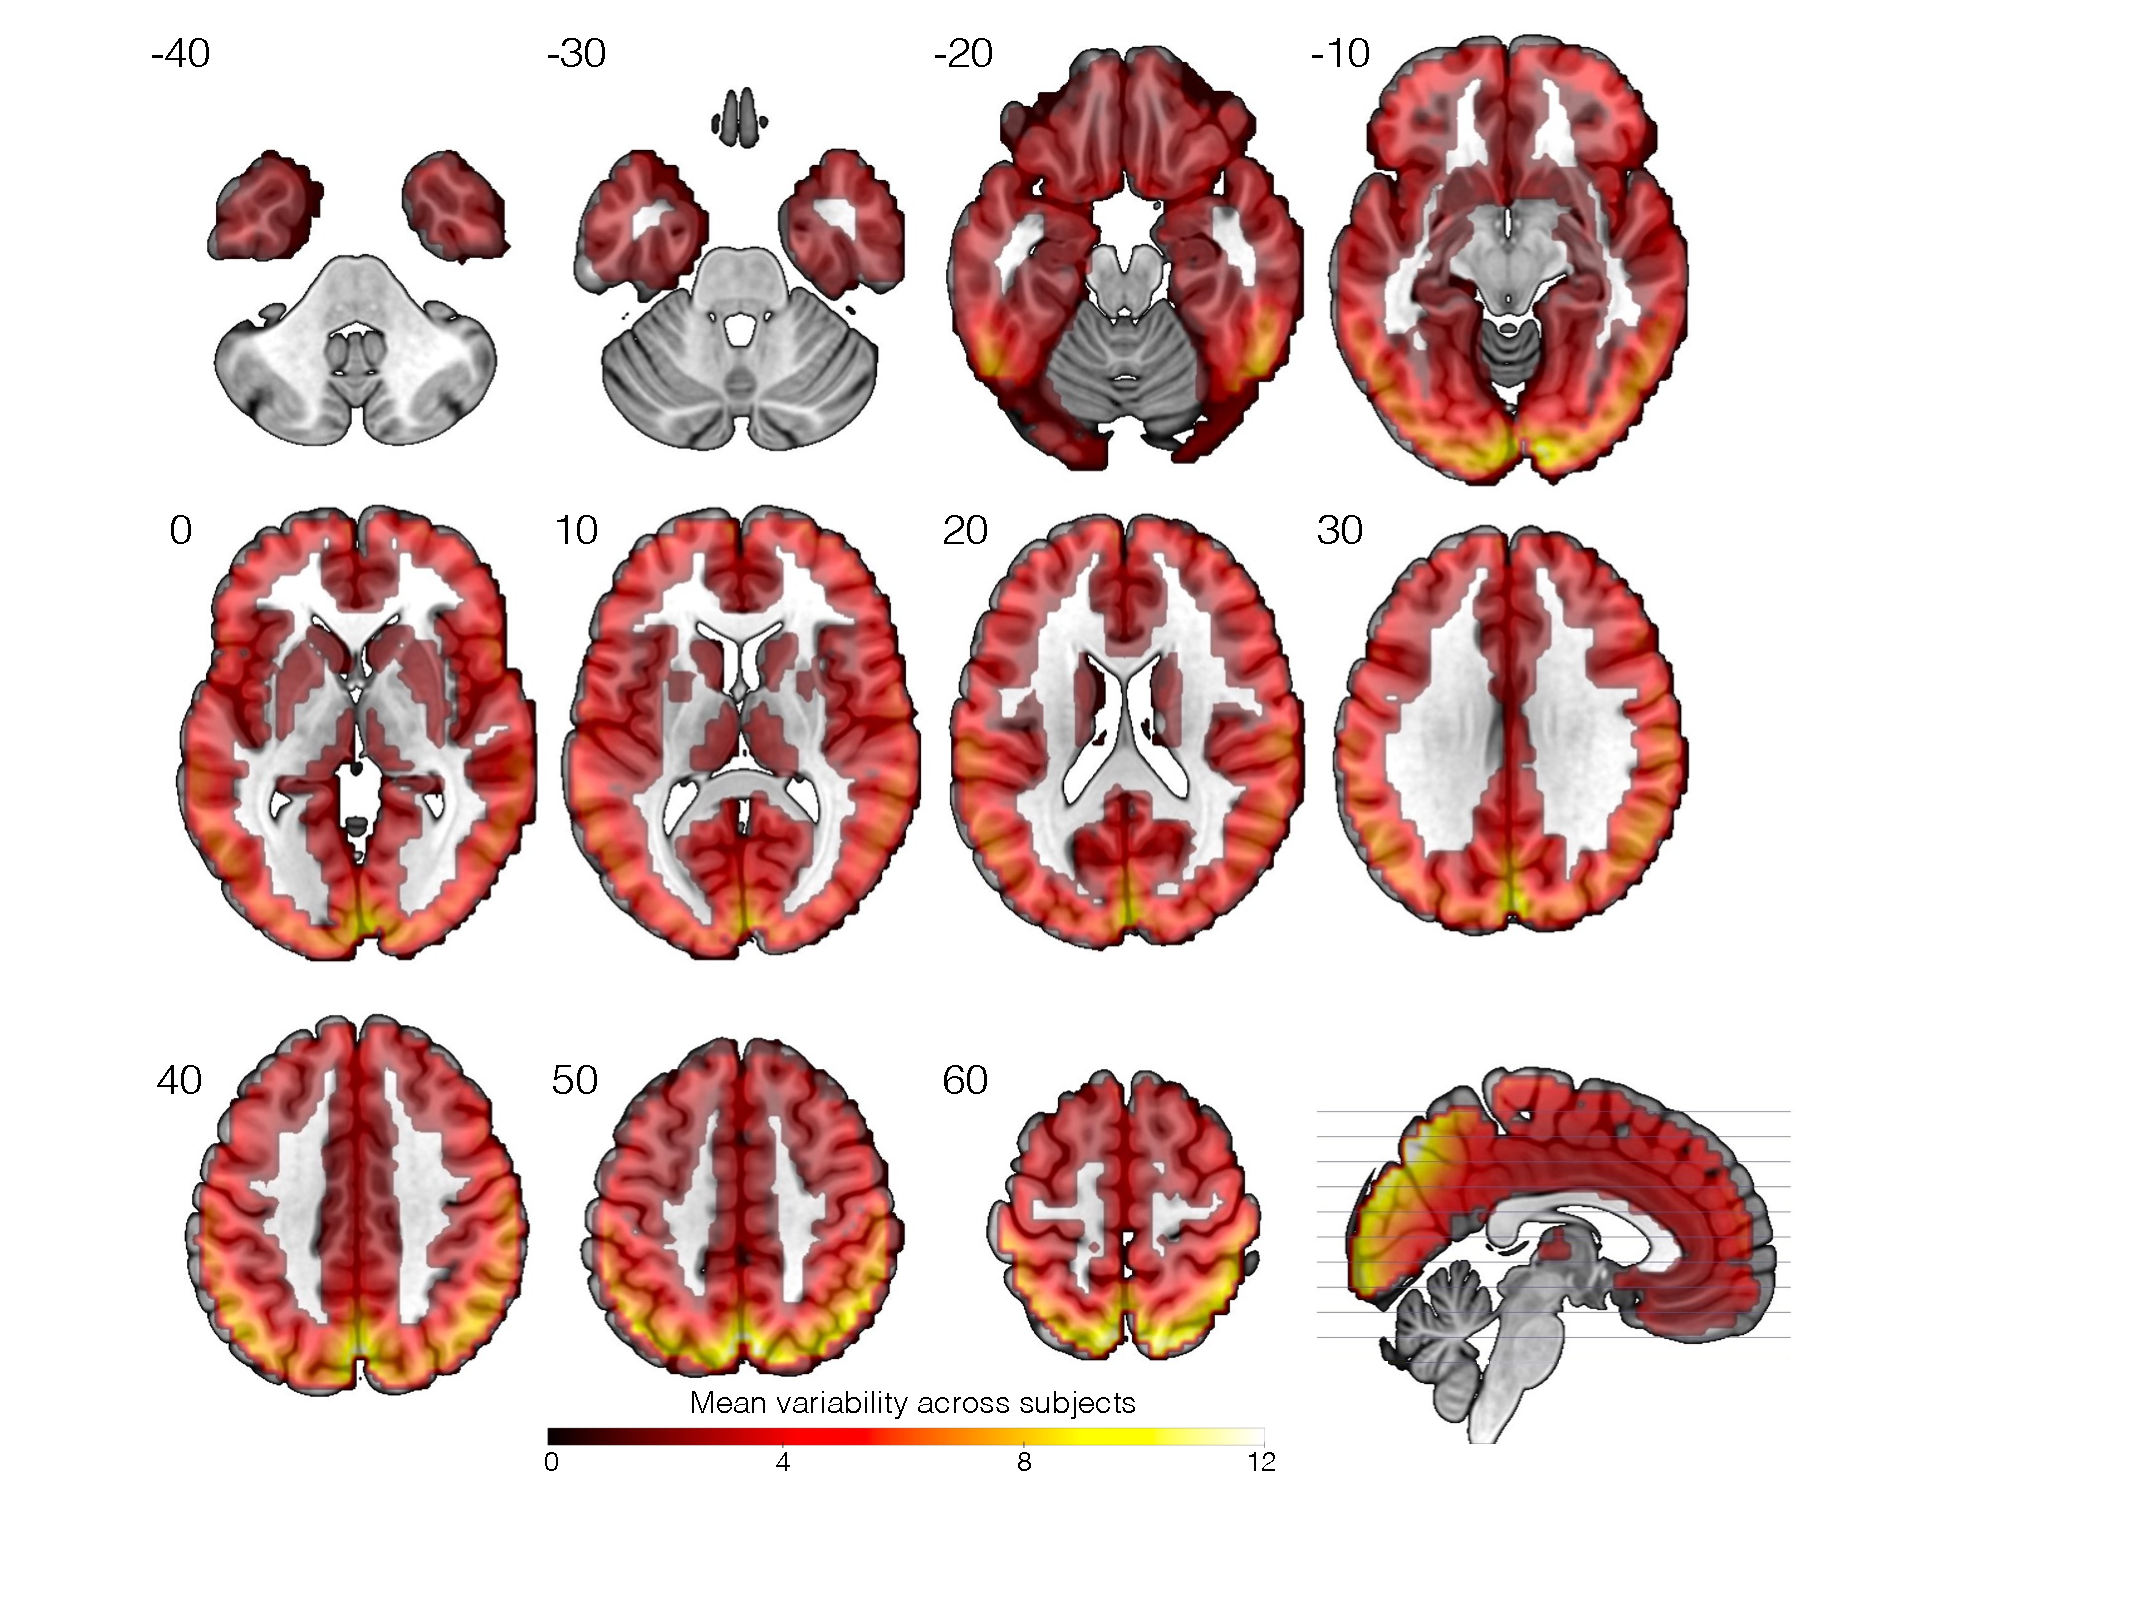
\includegraphics[width=0.9\linewidth]{Ch3/Fig1_meanVarMap.pdf}
\caption{\textbf{Mean variability map across the population. }  Calculated as the average of the standard deviation of the BOLD signals from each subject from both groups. Numbers on the top left indicate MNI coordinates in the Z axis. There was no significant difference between the mean variability maps of each group separately, as measured by Student's T-tests.}\label{fig:meanVarMap}
\end{figure}


\subsubsection*{BOLD variability evolves differently in preterm-born children} 
Figure \ref{fig:PLS_var} shows the brain and environment saliences for the significant latent component (p~=~0.006) yielded by the PLSC analysis. For fullterm-born children, there was a positive effect of GA and age, as well as an interaction between the two, on BOLD variability. This indicates that, as young adolescents grow older, and the longer they have spent in the womb, the more variability they will present in the regions shown in Figure \ref{fig:PLS_var}B. As for preterm-born children, contrary to their peers, age had a negative effect on BOLD variability, suggesting an altered trajectory for the development of this feature in this group. Moreover, although GA alone had no significant effect on BOLD variability, an interaction between GA and age did have a positive effect, suggesting that in older children, a longer gestation is linked to increased BOLD variability, bringing them closer to fullterm controls. The brain regions most implicated in the relationship uncovered by the significant latent component are shown in  Figure \ref{fig:PLS_var}B with a bootstrap ratio threshold of BSR = 3, which is equivalent to p-values less than 0.001.  In particular, the bilateral hippocampi (Hipp), insulae (Ins), ventral and dorsal anterior cingular cortex (ACC) all have a BSR < 6, which corresponds to a p-value less than 0.00001.



\begin{figure}[h!] 
\centering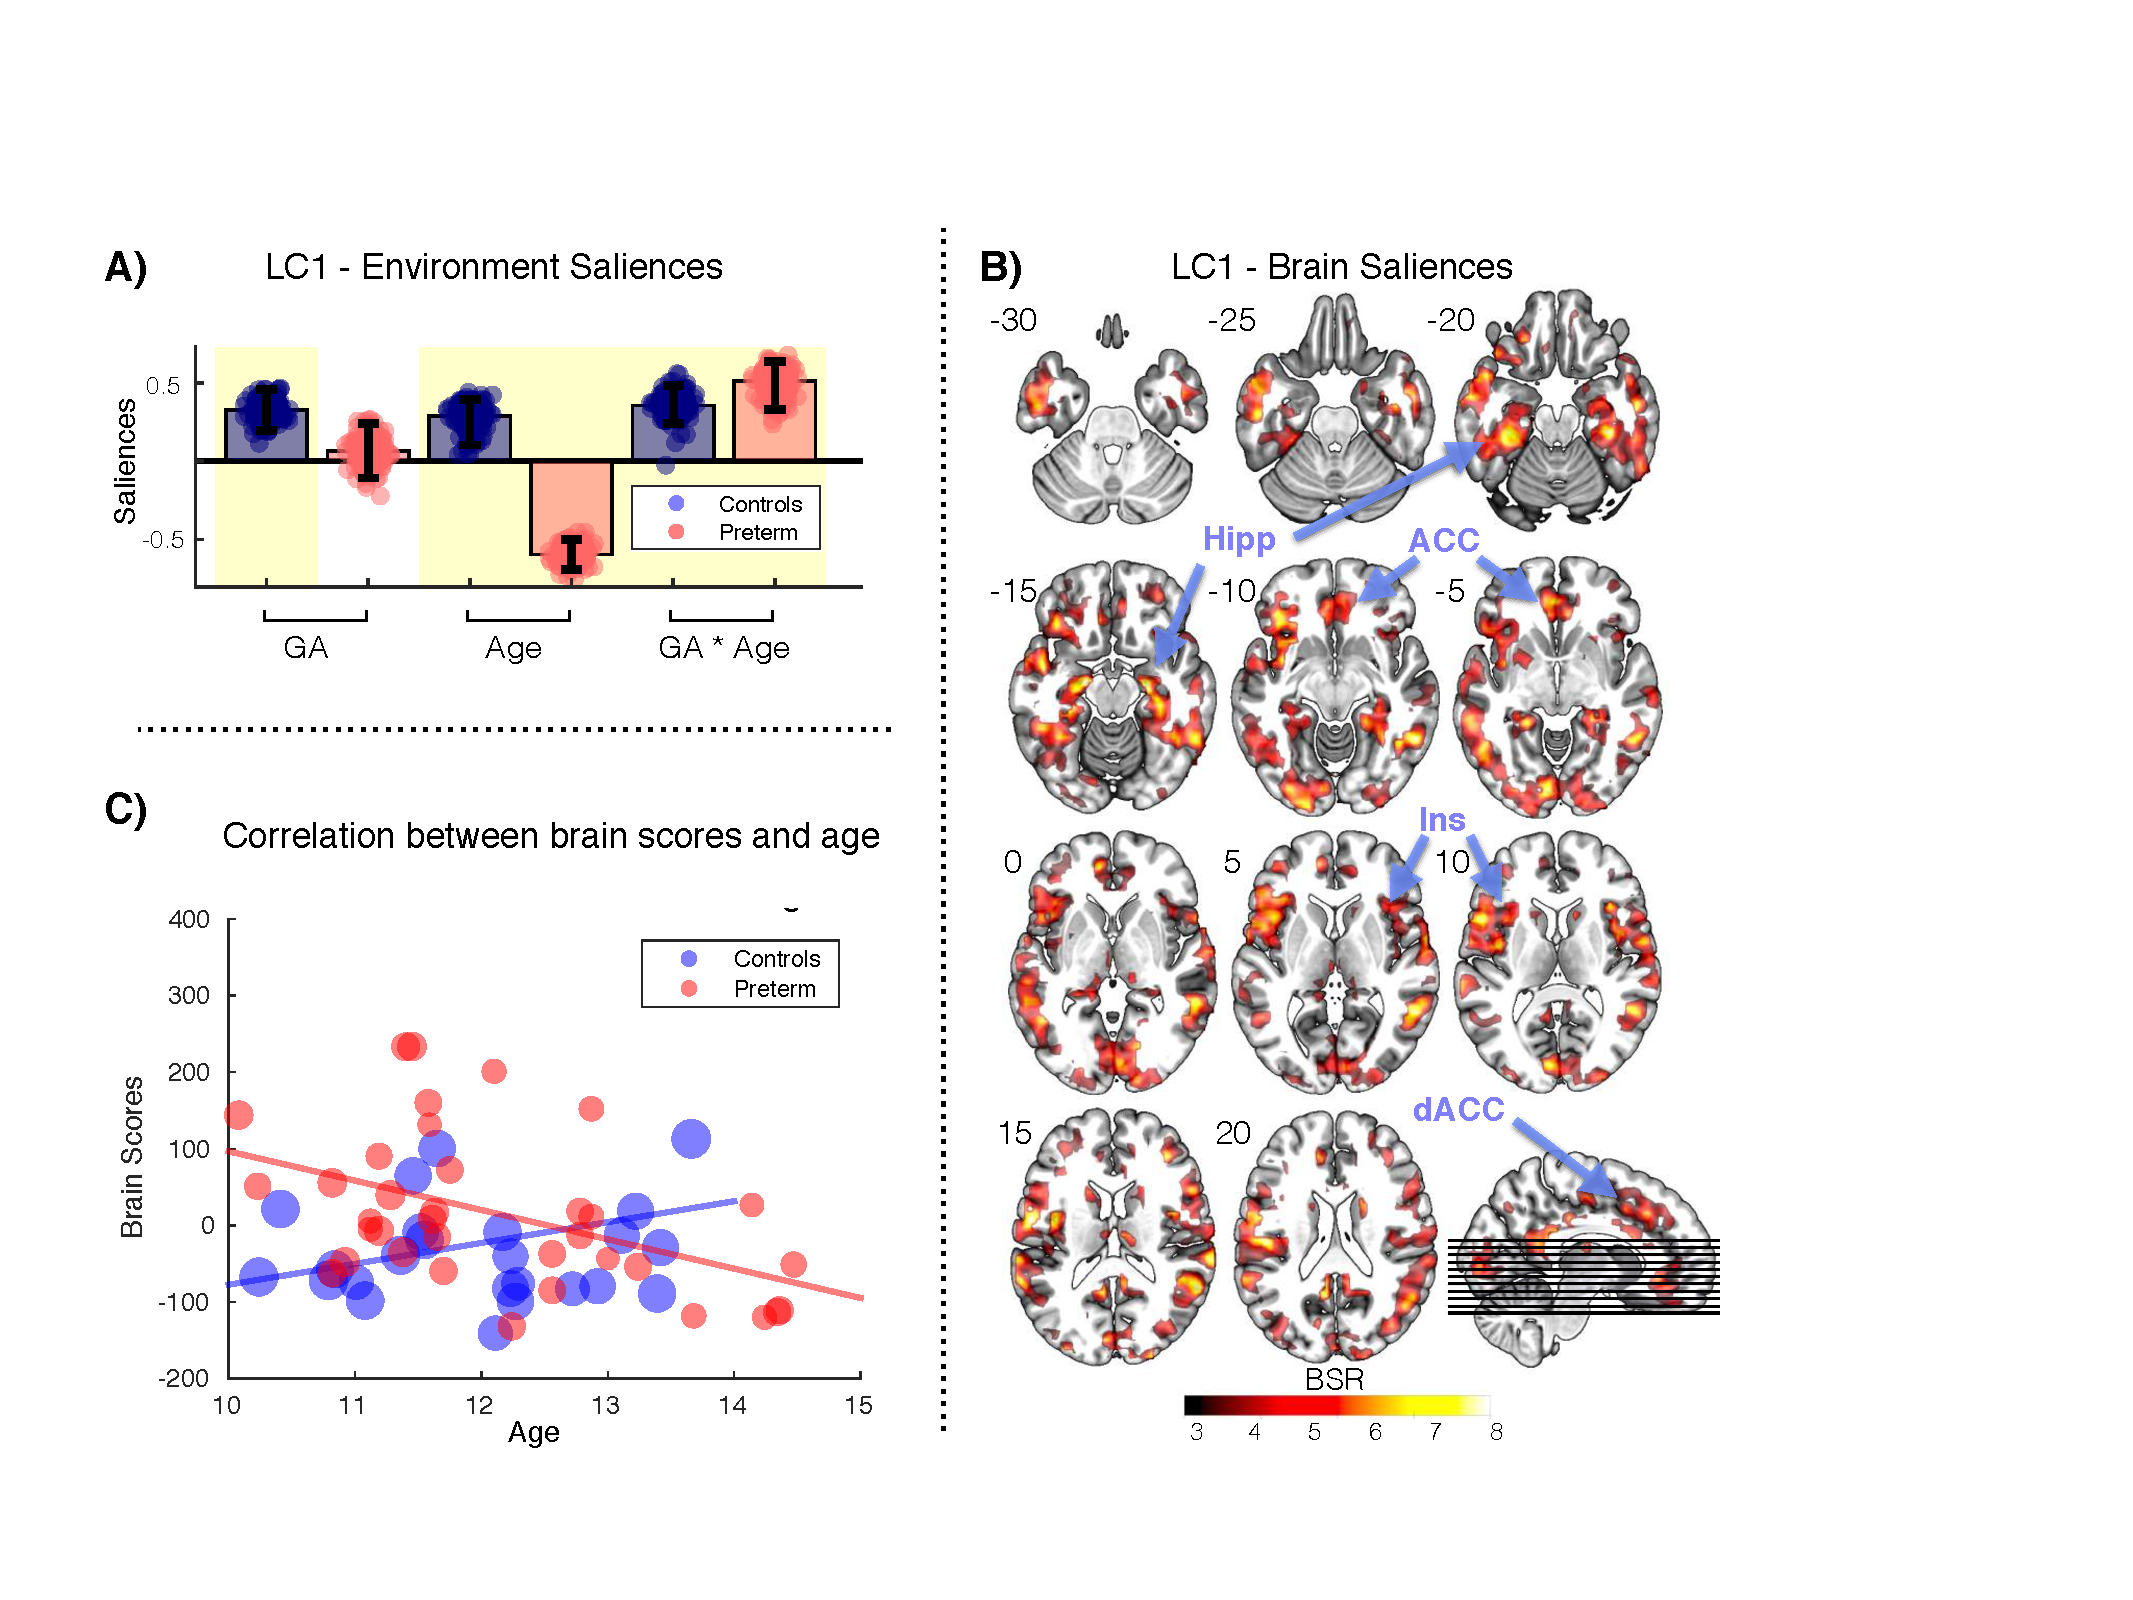
\includegraphics[width=1\linewidth]{Ch3/Fig2_PLS_var_LC1_20200205.pdf}
\caption{\textbf{BOLD variability and its link to environmental measures.} Partial least squares correlation (PLSC) results for BOLD variability and environmental measures for preterm-born young adolescents and full term born controls.  A)~Environment weights for latent component (LC) 1. GA = Gestational Age. Error bars correspond to bootstrapping 5th--95th percentiles. B)~Brain weights for LC 1. Numbers on the top left of each slice correspond to planes in Montreal Neurological Institute coordinates. C)~Correlations between brain scores and age in the two groups. For this plot, brain scores (Lx) were calculated using brain data normalised across all participants (as opposed to within-group), to allow group baselines to be compared. The size of each bubble is proportional to the corresponding subject's gestational age. %an eventual group effect in the baseline (typically ignored by PLS analyses) could have been identified
}. \label{fig:PLS_var}
\end{figure}



\subsubsection{Co-activation patterns}

Out of the brain areas highlighted in our BOLD variability analysis' results, the dorsal anterior cingulate cortex (ACC) has been previously reported to showcase alterations in both function and static connectivity in preterm-born individuals at various stages in life \citep{White2014,Daamen2015,Lordier2019}. We thus selected this region as a seed for further investigation using CAP analysis. 

\subsubsection*{ACC co-activates with typical resting-state networks in young adolescents} Consensus clustering was performed on K~=~2--20, and the lowest proportion of ambiguously clustered frames indicated K~=~6 as the ideal number of centroids for the clustering step. The co-activation patterns obtained correspond to well known resting-state networks and can be seen in Figure \ref{fig:CAPs}. CAP~1 corresponds to the default mode network (DMN), including the anterior medial prefrontal cortex, posterior cingulate cortex and angular gyri. CAP~2 includes the anterior cingulate cortex and the dorsolateral prefrontal cortex. CAP~3 corresponds to the dorsal attention network (DAN). CAP~4 includes nodes typically associated with the language network. CAP~5 includes the insula and dorsal ACC, nodes associated with the salience network (SN). Finally, CAP~6 corresponds to the visual network.


\begin{figure}[h]
\centering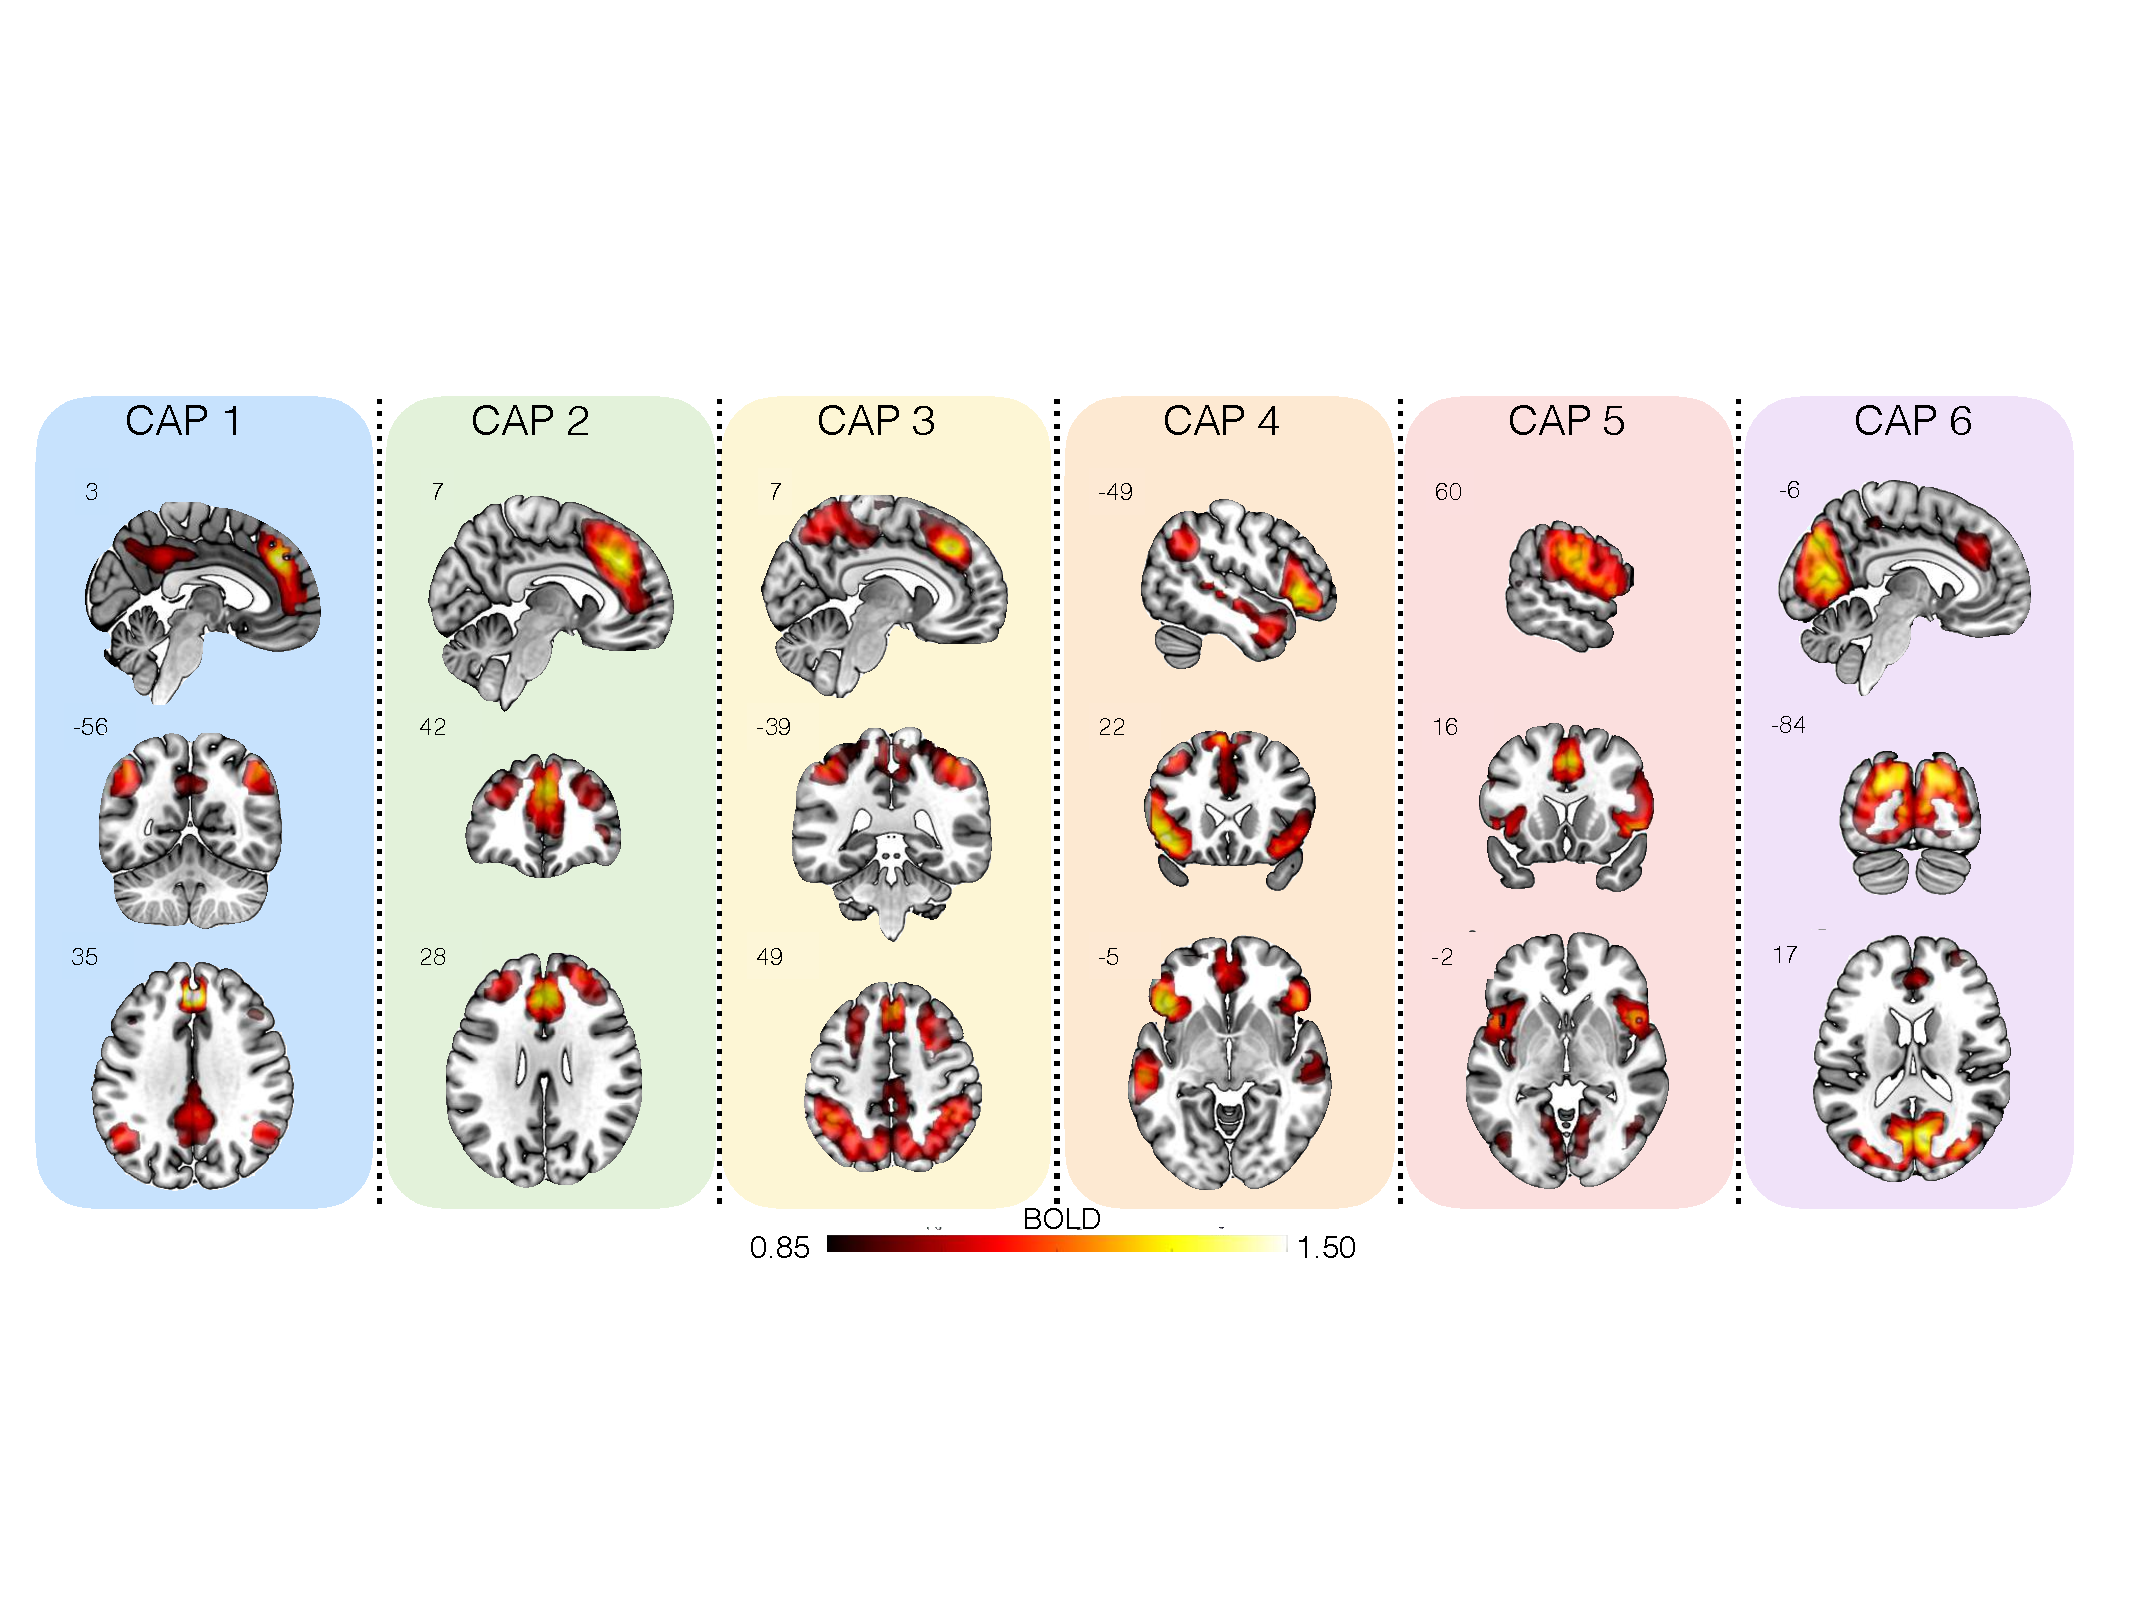
\includegraphics[width=1\linewidth]{Ch3/Fig3_CAPs_threshodled20200203.pdf}
\caption{\textbf{Spatial patterns of co-activation with the anterior cingulate cortex in young adolescents.} Co-activation Patterns (CAPs) were obtained from all subjects, including preterm-born young adolescents and fullterm controls. Numbers on the top left corner of slices correspond to Montreal Neurological Institute coordinates. Voxels were thresholded at 0.85, the same threshold used on the seed time course to keep 15\% of frames for clustering in the CAP analysis.  CAP~1 = default mode network ; CAP~2~=~anterior cingulate cortex and dorsolateral prefrontal cortex; CAP~3~=~dorsal attention network; CAP~4~=~language network; CAP~5~=~salience network; CAP~6~=~visual network.} \label{fig:CAPs}
\end{figure}




\subsubsection*{No group differences in individual CAP metrics between preterm- and fullterm-born participants} None of the individual CAP metrics we analysed (i.e.,  number of entries; average duration; number of transitions to and from baseline; and total number of occurrences) were significantly different between groups, as compared using two-sample t-tests ($p~>~0.05$, \textit{n.s.}). 

\subsubsection*{Altered trajectories of ACC-CAPs over time in preterm-born young adolescents} We then tested whether there were significant interplays between the six CAPs that were expressed differently between the two groups over time. To this end, we employed a PLSC analysis including the total number of occurrences per CAP and the environmental measures. We found one significant latent component (LC1, $p~=~0.001$) as shown in Figure \ref{fig:PLS_var}. Environment weights for LC1  indicate robust weights of gestational age (GA), age at assessment and an interaction of the two for preterm young adolescents, whereas age at assessment and its interaction with GA contributed robustly to LC1 in the control group (Fig. \ref{fig:PLS_CAPs}A). CAP occurrence saliences show that internally oriented networks such as the DMN have a positive weight in the relationship uncovered by LC1, while externally oriented networks (e.g., language, visual) are negatively weighted (Fig. \ref{fig:PLS_CAPs}B). The correlation plot between brain scores and age shows that this relationship is altered in preterm-born young adolescents as compared to their fullterm peers (Fig. \ref{fig:PLS_CAPs}C). Specifically, brain scores start lower for the VPT group at the age of 10, but increase at a higher pace than for the control group, eventually surpassing it. 



\begin{figure}[h]
\centering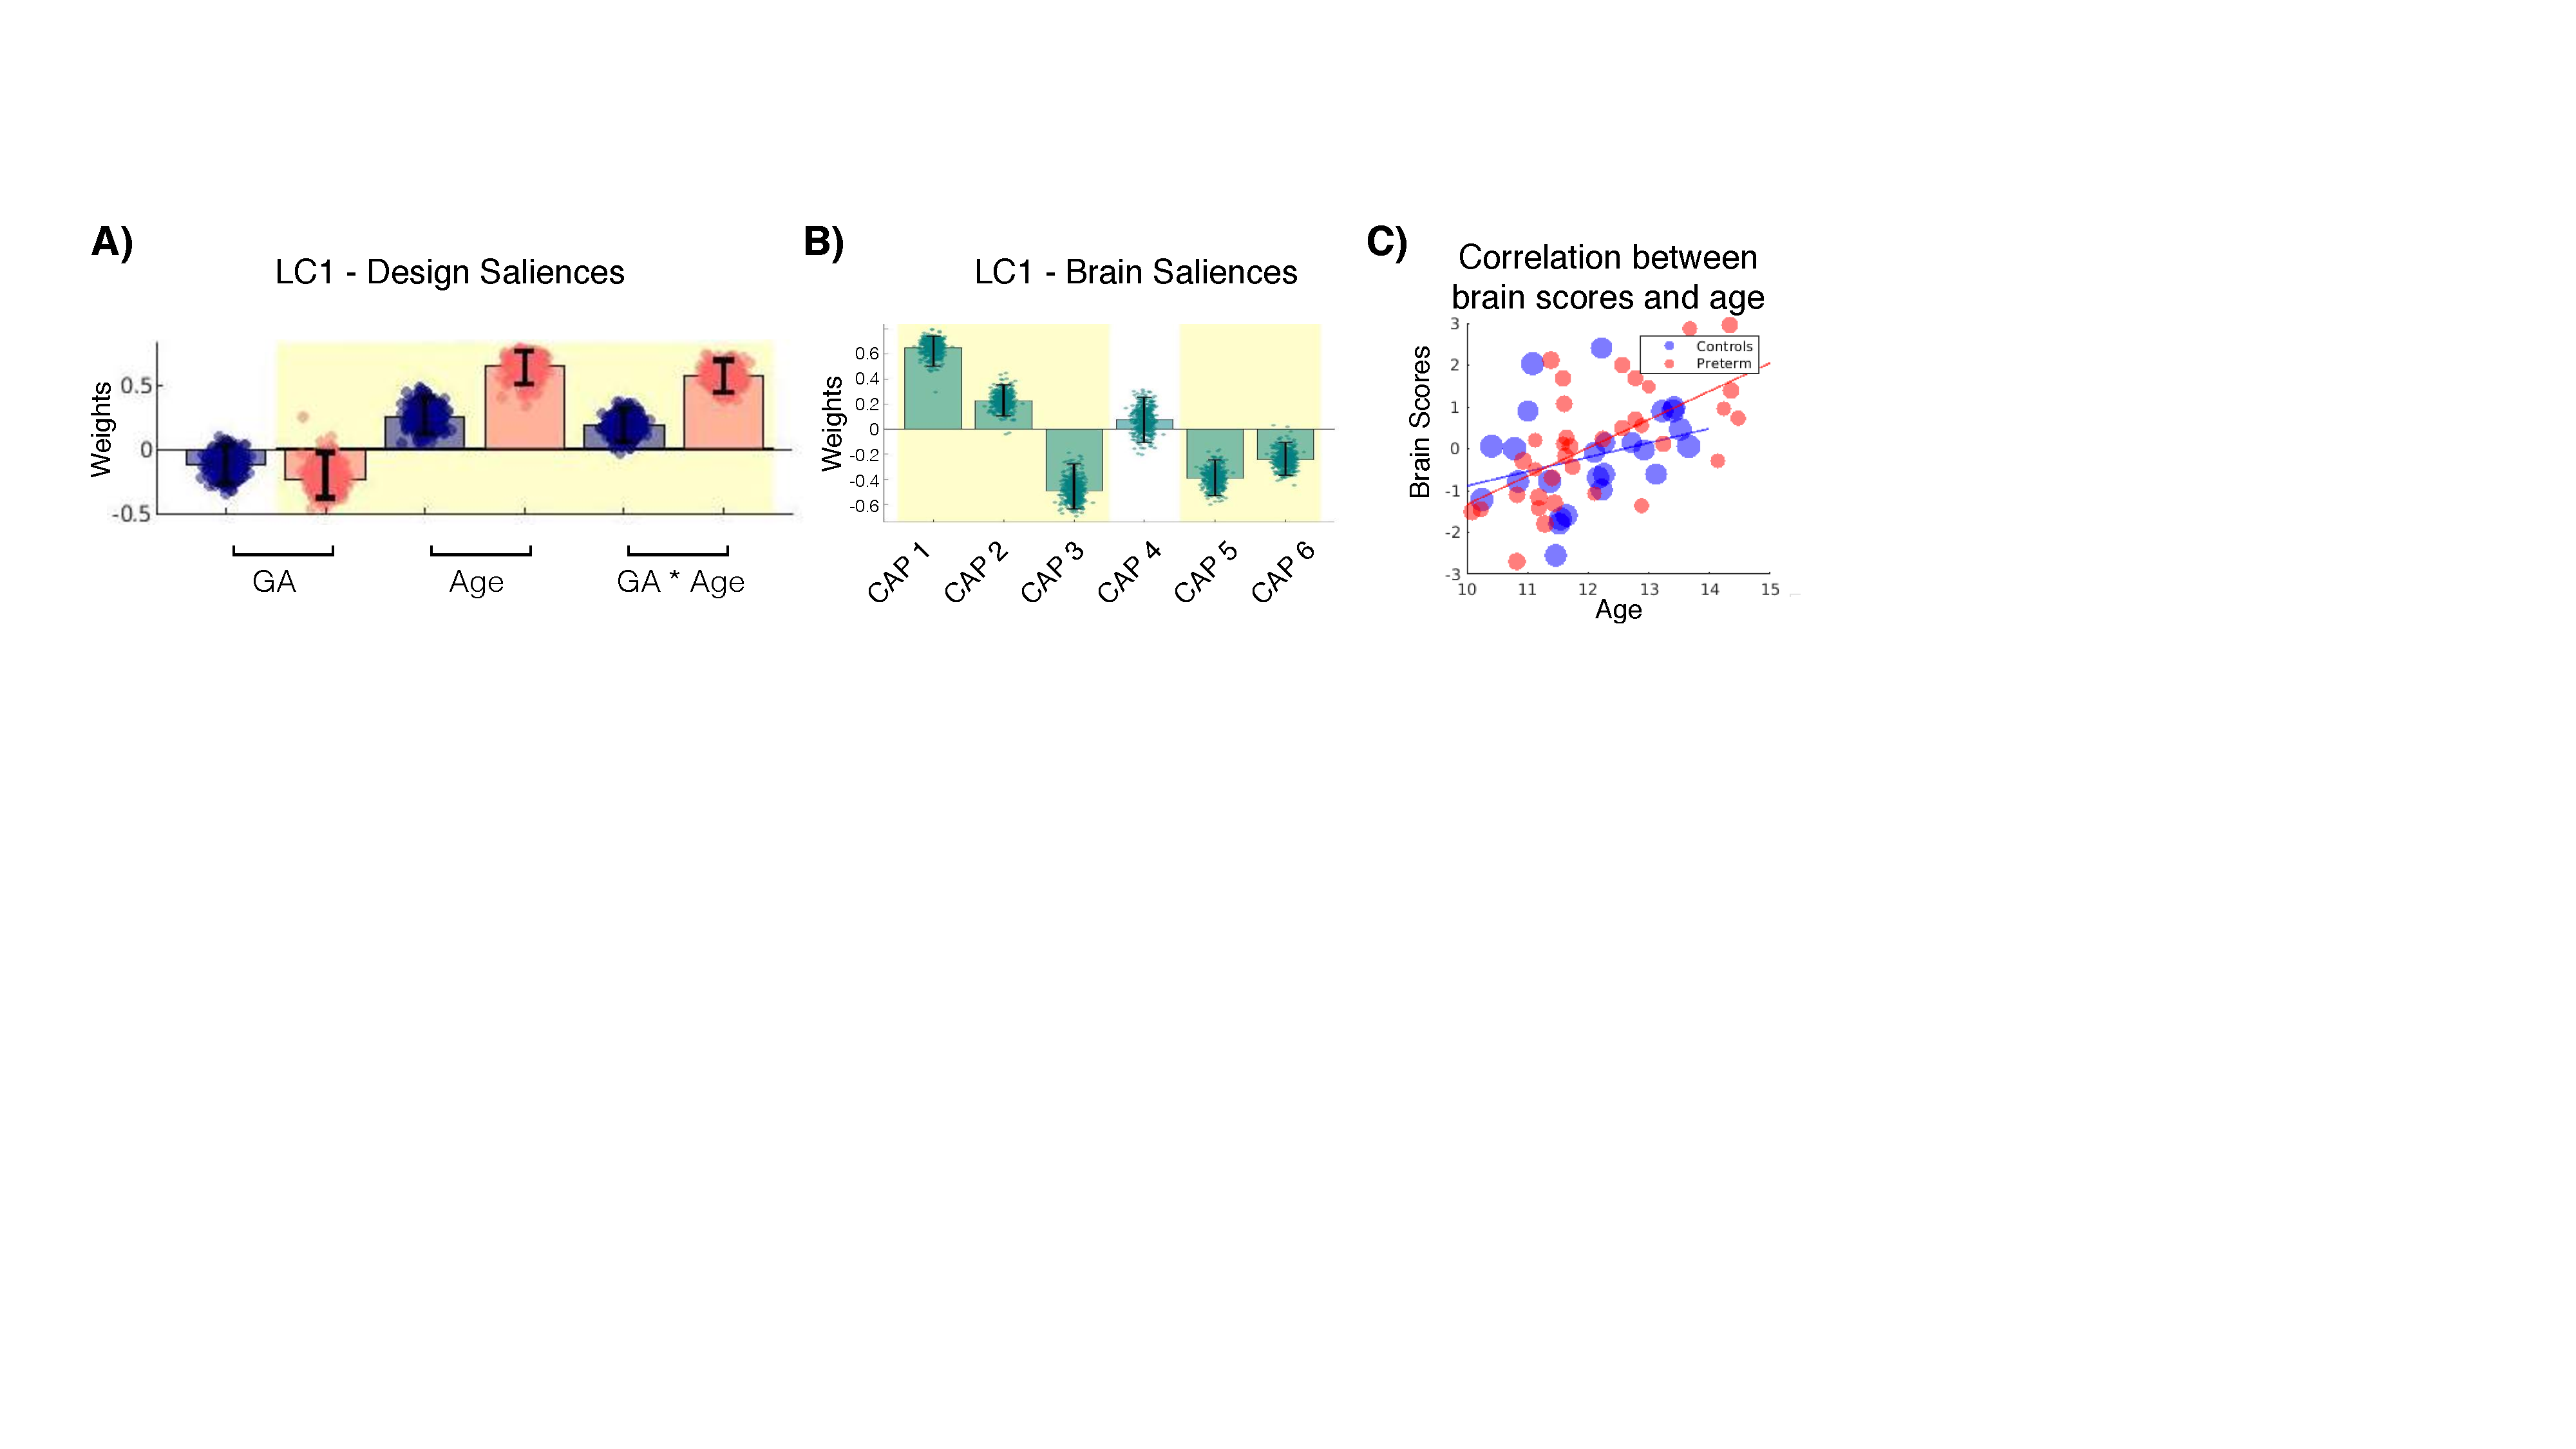
\includegraphics[width=1\linewidth]{Ch3/Fig4_CAPs_PLS_results_20200218.pdf}
\caption{\textbf{Altered trajectory of ACC-CAPs development over time in preterm-born young adolescents.} Partial least squares correlation between CAP occurrence and age-related measures lead to one significant latent component ($p~=~0.001$).   A)~Environment weights for LC1  indicate robust weights of gestational age (GA), age at assessment and an interaction of the two for preterm young adolescents (red bars), whereas age at assessment and its interaction with GA contributed robustly to LC1 in the control group (blue bars); blue bars represent fullterm controls. B)~CAP occurrence saliences show that internally oriented networks have a positive weight in the relationship uncovered by LC1, while externally oriented networks (e.g., language, visual) have a negative weight.  C)~The correlation plot between brain scores and age shows the different trajectories of CAP occurrence across age in the two groups.} \label{fig:PLS_CAPs}
\end{figure}




\subsection{Discussion}

This study investigated dynamic features of brain activity and connectivity in preterm-born young adolescents, with the particular goal of tracking their evolution during this phase of development. To the best of our knowledge, we were the first to investigate BOLD variability in this population.  We additionally employed co-activation pattern (CAP) analysis using a brain area known to be vulnerable in this population --- the dorsal anterior cingulate cortex --- as a seed to reveal several different spatial patterns, representing well-known resting-state networks, that dynamically co-activate with this ROI over time. Finally, we revealed that the development of both BOLD variability and the balance between CAPs is altered in VPT young adolescents as compared to fullterm controls. 


\paragraph{Altered BOLD variability evolution in the Very Preterm}
BOLD variability is broadly altered in the preterm group, for which we found a negative effect of age as compared to a positive effect within the control group (Fig. \ref{fig:PLS_var}A). Of note, the pattern of alterations includes large parts of the DMN such as the medial prefrontal cortex and the posterior prefrontal cortex. \cite{Garrett2011} found differences in a similar set of regions when studying BOLD variability in healthy adults during the performance of a task, with the elderly, low performing group showing decreased variability. Importantly, the posterior cingulate cortex and precuneus have been singled-out as functional and structural network hubs, linked to theory-of-mind and self-referential processes \citep{Spreng2009,VandenHeuvel2013}, both of which are affected in the preterm-born\cite{} \add{add reference}. In pre-adolescents, a recent study in normative functional connectivity development found that FC within the DMN was anti-correlated with age and cognitive performance \citep{Jiang2018}. The increase in BOLD variability with age in the same regions in our fullterm group aligns with the idea that variability at the right level is necessary to yield a greater dynamic range and complexity, allowing flexibility in brain function and connectivity \citep{McIntosh2010,Deco2011,Garrett2013b}.
Along these lines, development of variability seen in the preterm group may be linked to other functional and behavioural alterations seen in this group. For instance, exacerbated variability in the medial prefrontal cortex in ADHD patients aged 9.91$\pm$1.24 (as compared to typically developing children) is strongly correlated with the severity of ADHD symptoms and inattention \citep{Nomi2018}. The positive effect of the interaction between gestational age and age in our preterm group shows a similar relationship between BOLD variability and prematurity in our younger preterms (Fig. \ref{fig:PLS_var}A, B). In particular, the fact that variability is higher in the preterm group at an early age and gradually decreases past the fullterm point may indicate a compensation mechanism that overshoots, and thus does not reach ideal levels (e.g., comparable to typically developing controls) within this period of life. It would be interesting to follow up this study with a BOLD variability analysis in preterm-born adults to check if, like with other brain measures and behavioural traits, the alterations last throughout life.

The pattern of BOLD variability alterations includes other brain regions such as the bilateral hippocampus/amygdala and the insula – areas involved in a variety of functions ranging from affective processing to higher level cognition \citep{Uddin2018}. These regions have been previously found to be affected in the young preterm population, with accounts of altered developmental trajectories \citep{Thompson2014}, volumetry \citep{Chau2019}, and function \citep{Nosarti2006}. In general, our results agree with research showing that insular BOLD variability increases linearly with age in the resting state \citep{Nomi2018} in typically developing individuals, and show that this trajectory is altered in the preterm group. In our group comparison, there was no evidence of the previously found cortical-subcortical dichotomy in which BOLD variability increases with age in subcortical areas as opposed to cortical areas \citep{Garrett2013b}. This may be partly due to the fact that Garrett's study was performed using a task-based design. More importantly, PLSC extracts the multivariate pattern that most differentiates the two groups, suggesting a complex pattern of development alterations in the preterm group.


\paragraph{Altered ACC connectivity pattern in the Very Preterm}
To further understand the effects of BOLD variability and relate it to conventional functional connectivity, we investigate how the patterns of activation of the dorsal ACC --- a region that has been previously shown to be compromised in the preterm-born  \citep{White2014, Daamen2015, Lordier2019} --- relate to other areas in the brain. In keeping with our interest in the dynamic aspects of brain function, we chose to perform a co-activation patterns analysis to achieve this, retrieving 6 CAPs that included well known resting-state networks. There was no difference between the two groups when we compared the number of occurrences of each CAP individually. However, a multivariate analysis showed that the occurrence of certain combinations of CAPs developed differently in the two groups. Of note, the difference was mainly driven by number of entries in each state, as opposed to the duration of each brain state. \cite{Sherman2014} found that DMN integration increased from ages 10 to 13 in typically developing children, and segregation between the DMN and dorsal attention networks increased (i.e., the between-network correlations weakened). This is in line with what we found in our control group. Interestingly, the preterm group follows the same trend, but in a much more accentuated way. Similarly to our results on BOLD variability, this suggests that there is a mechanism in place that fails to identify the optimal point of balance and thus overshoots.  \cite{Nosarti2006} found that, in preterm adults, a weaker connectivity in the salience network (which includes the dorsal ACC and the insula) is related to worse outcomes, which is in line with our result that, in the preterm group, co-occurrence of the ACC and the insula decreases more rapidly than in the control group.  These findings, combined, further highlight early adolescence as a significant time for maturation of the brain's functional architecture, and corroborate the idea this development fails to find the optimal compensatory balance that preterm-born individuals.


Interestingly, the combinations of patterns whose co-occurrence with the ACC found in our CAPs analysis reveals a dichotomy between the occurrences of internally- (i.e., DMN, mPFC) versus externally-oriented (i.e., DAN, visual) networks \citep{Zabelina2016}. Internally-oriented cognition comprises creative thinking; making social inferences; prospection; and mind-wandering \citep{Zabelina2016, Buckner2019}. Networks which support externally-oriented cognition, in turn, are typically involved in language; visual; and somatosensory tasks, attention regulation, and are usually positively correlated at rest \citep{Lee2012}, in line with our results. A study on resting-state functional connectivity including young adolescents aged 10--16 found that very preterm participants showed weaker connectivity in externally-oriented networks such as the visual and DAN \citep{Wehrle2018}. The results considered the groups in a categorical way, but includes a slightly older population than ours. This could explain the finding of a weaker task-oriented network connectivity in preterm as compared to controls, which in line with what is seen in our older participants. This weakened connectivity has also been found in adult preterm-born individuals aged 28 and above \citep{White2014}. Our study thus provides complementary insight into the trajectory of the differences seen between the two groups, and suggests that the disconnectivity seen in later life stages may be related to faulty compensation mechanisms that start during the highly dynamic age range of early adolescence.


\subsubsection*{Conclusions}
Our study shows for the first time that the trajectory of BOLD signal variability development is altered in young adolescents born prematurely, and that these alterations follow a broad spatial pattern in the brain comprising regions previously found to be affected by preterm birth. The previous implication of the brain areas observed in our study in preterm birth and cognitive performance suggests exploring the relationship between the development of BOLD signal variability and behavioural outcomes as a promising avenue for further research. In addition, we explored the development of dynamic functional connectivity in this populating by examining how the interplay between different multivariate co-activation patterns changes with age. We found that the change in the balance between  internally- and externally-oriented networks across age is more accentuated in the preterm group. Taken together, our observations suggest that the preterm-born brain triggers neurological compensation mechanisms that start during the highly dynamic age range of early adolescence and fail to find an optimal balance. 





\subsection*{Acknowledgements}
This work was supported by the Swiss National Science Foundation, grant no. 324730-163084 to PSH. The authors thank Loan Mattera, Roberto Martuzzi and Greta Mikneviciute for their help in data acquisition. 

\subsection*{Conflict of Interest Statement}
The authors declare that the research was conducted in the absence of any commercial or financial relationships that could be construed as a potential conflict of interest.








\begin{comment}
In this chapter we will see some examples of tables and figures.

\section{Tables}
Let's see how to make a well designed table.

\begin{table}[tb]
\caption[A floating table]{A floating table.}
\label{tab:esempio}
\centering
\begin{tabular}{ccc}
\toprule
name & weight & food \\ 
\midrule
mouse	& 10 g	& cheese \\
cat	& 1 kg	& mice \\
dog	& 10 kg	& cats \\
t-rex	& 10 Mg	& dogs \\
\bottomrule 
\end{tabular}
\end{table}

The table~\ref{tab:esempio} is a floating table and was obtained with the following code:
\begin{lstlisting}
\begin{table}[tb]
\caption[A floating table]{A floating table.}
\label{tab:example}
\centering
\begin{tabular}{ccc}
\toprule
	name 	& weight & food	  \\ 
\midrule
	mouse	& 10  g	 & cheese \\
	cat		&  1 kg	 & mice	  \\
	dog		& 10 kg	 & cats   \\
	t-rex	& 10 Mg	 & dogs	  \\
\bottomrule 
\end{tabular}
\end{table}
\end{lstlisting}

\lipsum[1-2]


\section{Figures}
Let's see now how to put one or several images in your text.


\begin{figure}[tb] 
\centering 
\includegraphics[width=0.5\columnwidth]{galleria_stampe} 
\caption[A floating figure]{A floating figure (the lithograph \emph{Galleria di stampe}, of M.~Escher, got from \url{http://www.mcescher.com/}).}
\label{fig:galleria} 
\end{figure}

\begin{figure}[tb] 
\centering 
\includegraphics{some_vector_graphics} 
\caption[A floating figure]{A floating figure with text typeset in "Utopia Latex", a font provided in the template-folder for typesetting figures with greek characters. The text has been "outlined" for best compatibility with the repro during the printing.}
\label{fig:vector_graphics} 
\end{figure}


The figure~\ref{fig:galleria} is a floating figure and was obtained with the following code:
\begin{lstlisting}
\begin{figure}[tb] 
\centering 
\includegraphics[width=0.5\columnwidth]{galleria_stampe} 
\caption[A floating figure]{A floating figure ... }
\label{fig:galleria} 
\end{figure}
\end{lstlisting}


\lipsum[1-2]

\begin{figure}[tb]
\centering

\subfloat[Asia personas duo.]
{\includegraphics[width=.45\columnwidth]{lorem}} \quad
\subfloat[Pan ma signo.]
{\label{fig:ipsum}%
\includegraphics[width=.45\columnwidth]{ipsum}} \\
\subfloat[Methodicamente o uno.]
{\includegraphics[width=.45\columnwidth]{dolor}} \quad
\subfloat[Titulo debitas.]
{\includegraphics[width=.45\columnwidth]{sit}}
\caption[Tu duo titulo debitas latente]{Tu duo titulo debitas
latente.}
\label{fig:esempio}
\end{figure}

The figure~\ref{fig:esempio} is a floating figure and was obtained with the following code:
\begin{lstlisting}
\begin{figure}[tb]
\centering
\subfloat[Asia personas duo.]
{\includegraphics[width=.45\columnwidth]{lorem}} \quad
\subfloat[Pan ma signo.]
{\label{fig:ipsum}%
\includegraphics[width=.45\columnwidth]{ipsum}} \\
\subfloat[Methodicamente o uno.]
{\includegraphics[width=.45\columnwidth]{dolor}} \quad
\subfloat[Titulo debitas.]
{\includegraphics[width=.45\columnwidth]{sit}}
\caption[Tu duo titulo debitas latente]{Tu duo titulo debitas latente.}
\label{fig:esempio}
\end{figure}
\end{lstlisting}


\lipsum[3-8]

\end{comment}